\chapter{Анализ предметной области}
% выбор направления исследований, включающий обоснование направления исследования,
% методы решения задач и их сравнительную оценку
% описание выбранной общей методики проведения НИР;

Ну шо, бандиты, давайте сначала рассмотрим, какие игры мы тут будем разбирать. Сначала дам вам названия игр, а потом расскажу, какие проблемы с ними связаны и что за игры это такие.
Все игры, о которых мы говорим, связаны с Марковскими играми (\ref{sec:markov-games}), но это уже в конце подробно расписано.
Так что, понимайте, что для нашей темы искусственного интеллекта в играх, мы юзаем математические модели, которые формализуют всю эту срань.
А вот сейчас ниже я сформулирую все это формально-официально, чтоб вы четко поняли, как тут все устроено.
Что касается НИР, то тут нам надо выяснить, какие методы решения задач применимы и какие критерии надо учитывать. Потом будем сравнивать эти методы, но это уже позже.

%%%%%%%%%%%%%%%%%%%%%%%%%%%%%%%%%%%%%%%%%%%%%%
\section{Типы игр, чуваки}

Алё, тут мы разберем три типа игр, понятно? Ну давайте, расскажу о каждом типе по подробнее.

\subsection{Кооперативные игры}

Вообще, в таких играх все хавки разделяют общий бонус, понимаешь? Это же те самые MDP с несколькими агентами (MMDP), если ты в теме. И в таких играх все Q-функции и V-функции агентов на одной волне, братан. Идеальная тактика для каждого хавка - это тактика всех хавков вместе. Кстати, если хочешь, можешь использовать Q-учение для этого. А потом Нэша достигнешь.

Но бывает, что для каждого хавка награда своя. И тогда награда для команды - это средняя из наград каждого хавка. Это называется decentralized MARL, если хочешь знать. И тут каждый хавк сам за себя, понимаешь? Интересно, что они могут изобрести свой язык общения, чтобы выстроить идеальную тактику вместе.

\subsection{Соревновательные игры}

Такие игры обычно моделируют как игры с нулевой суммой, а понимаешь? То есть, если все сложить, получится ноль. В основном в таких играх два игрока участвуют. Ну а Нэш здесь описывает тактику, которая позволяет минимизировать самую хуёвую награду на долгой дистанции. Понимаешь, братан?

\subsection{Смешанные игры}

Еще есть игры с общей суммой, а понимаешь? Они же general sum games. В таких играх сумма наград хавков может быть любой и все зависит от взаимодействия между ними.


\section{Проблемы, блядь, когда применяешь этот хуевый метод к игровому искусственному интеллекту}

Когда мы хуячим методы обучения с подкреплением на игровой искусственный интеллект, то натыкаемся на следующие проблемы:
\begin{itemize}[label=---]
	\item комбинаторная сложность, блядь, --- размер пространства действий растет экспоненциально, как хуевая мамаша, с увеличением числа агентов;
	\item оптимизируемые величины многомерны, блядь, --- не можем выразить нашу умственную мастурбацию одной хуевой метрикой;
	\item проблема нестабильности, блядь, --- агенты, которые являются частью этого говна, обучаются в одиночку, хуячат свою хуиту и не общаются друг с другом, как две бляди на улице, а динамика этого дерьма постоянно меняется.
	\item редкая награда, блядь, --- награда прилетает только в конце игры, как хуевый бомж, который ждет благотворительности на свою хуиту.
\end{itemize}

\section{Рассматриваемые игры, блядь}

Мы, блядь, смотрели на разные игры, которые являются смешанными, как хуевый коктейль. На этом говне мы потратили свое время:
\begin{itemize}[label=---]
	\item Проблемы повторяющихся матриц (Matrix Games), блядь, --- это такие игры, где награды описываются матрицами, как хуевой математический график. Они усложнены тем, что есть хуевый локальный минимум на пути к эквилибриуму;
	\item Частицы с несколькими агентами (MPE), блядь, \ref{fig:mpe} --- это хуевые двумерные проблемы навигации, как хуевой штурман на корабле: Штурман-Искатель, Разносчик, Советчик, Жертва-Хищник;
	\item StarCraft (SMAC), блядь, --- это говно из компьютерной игры StarCraft с несколькими агентами, как хуевая бойня на экране;
	\item Level Based Foraging (LBF) --- а вот здесь агенты должны грызть еду на карте, чтоб выжить;
	\item Robotic Warehouse (RWARE) --- а вот в этой игре агенты должны тащить вещи до точки назначения и потом вернуться на базу.
\end{itemize}

\begin{figure}[H]
	\begin{center}
		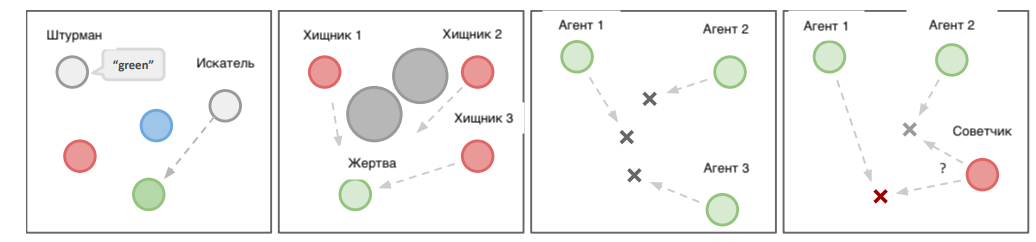
\includegraphics[pages=-, width=140mm]{./inc/img/mpe.png}
		\caption{Среды MPE, слева--направо: Штурман говорит Искателю к какой точке идти, Жертва скрывается от Хищников в серое убежище, Разносчики идут по разным местам, Советчик координирует Разносчиков.}
		\label{fig:mpe}
	\end{center}
\end{figure}

Таблицы \ref{tab:games1} и \ref{tab:games2} сравнивают игры по разным критериям.

% Please add the following required packages to your document preamble:
\begin{table}[H]
	\centering
	\caption{Сравнение игр по наблюдаемости и количеству наград}
	\label{tab:games1}
	\begin{tabular}{@{}|l|l|l|@{}}
		\toprule
		Игра           & Наблюдаемость     & Кол--во наград \\ \midrule
		Матричные игры & Полная            & Много          \\
		MPE            & Полная / Неполная & Много          \\
		SMAC           & Полная / Неполная & Много          \\
		LBF            & Полная / Неполная & Крайне мало    \\
		RWARE          & Полная / Неполная & Крайне мало    \\ \bottomrule
	\end{tabular}
\end{table}

% Please add the following required packages to your document preamble:
% \usepackage{booktabs}
\begin{table}[H]
	\centering
	\caption{Сравнение игр по сложности и количеству агентов}
	\label{tab:games2}
	\begin{tabular}{@{}|l|l|l|@{}}
		\toprule
		Игра           & \# агентов & Главная сложность             \\ \midrule
		Матричные игры & 2          & Не оптимальный эквилибриум    \\
		MPE            & 2--3       & Нестационарность              \\
		SMAC           & 2--10      & Большое пространство действий \\
		LBF            & 2--4       & Координирование               \\
		RWARE          & 2--4       & Крайне мало наград            \\ \bottomrule
	\end{tabular}
\end{table}

\section{Формализация}

Изложенные выше игры формализуются математическим языком согласно \cite{DBLP:journals/corr/abs-2011-00583} с помощью понятия Марковских игр.
Ниже представлены описания некоторых важных функций, используемых для решения игр.
Решение подразумевает поиск оптимальной стратегии. Определение оптимальной стратегии использует эти функции.

В последующих разделах под функцией будет подразумеваться нейросеть.

\subsection{Марковский процесс принятия решений} \label{sec:mdp}

Для среды с одним агентом Марковский процесс принятия решений (MDP) задается кортежем \( (\mathcal{S}, \mathcal{A}, \mathcal{P}, R, \gamma )\), элементы которого определяются следующим образом:

\begin{itemize}[label=---]
	\item \(\mathcal{S}\) --- множество состояний среды;
	\item \( \mathcal{A} \) --- множество действий агента;
	\item \( \mathcal{P}: \mathcal{S} \times \mathcal{A} \times \mathcal{S} \mapsto [0, 1] \) --- вероятность перехода из состояния \( s \in \mathcal{S} \) в состояние \( s' \in \mathcal{S} \) при выполнении действия \( a \in \mathcal{A} \);
	\item \( R: \mathcal{S} \times \mathcal{A} \times \mathcal{S} \mapsto R^1 \) --- награда за совершение действия \( a \in \mathcal{A} \) в состоянии \( s \in \mathcal{S} \) и переход в состояние \( s' \in \mathcal{S} \);
	\item \( \gamma \in [0, 1] \) --- коэффициент дисконтирования, влияет на вероятность предпочтения немедленной награды награде в будущем.
\end{itemize}

На каждом щелчке агент смотрит, что там за пиздец в среде \(s_t\) в момент времени \(t\) и принимает действие \(a_t\)

Решением задачи является стратегия \( \pi \) и от того, что агент ранее юзал (то есть от самого себя). Эта стратегия пытается достать максимально возможную хуйню, которая рассчитывается по формуле Беллмана.

\begin{equation}
	\pi(s) = \arg\max_{a \in \mathcal{A}} \mathbb{E} \left[ \sum_{t=0}^{\infty} \gamma^t R(s_t, a_t, s_{t+1}) \mid a_t \sim \pi(\cdot \mid s_t), s_0 \right].
	\label{eq:Q}
\end{equation}


Определим Q-функцию\footnote{Какую награду можно ожидать, если на шаге t выполним действие a, а дальше будем придерживаться стратегии?} и V-функцию значений\footnote{Какую награду можно ожидать, если будем придерживаться лучших действий согласно стратегии?} как:

\begin{equation}
	Q^{\pi}(s, a) = \mathbb{E} \left[ \sum_{t=0}^{\infty} \gamma^t R(s_t, a_t, s_{t+1}) \mid a_t \sim \pi(\cdot \mid s_t), s_0 = s, a_0 = a \right],
	\label{eq:V}
\end{equation}


\begin{equation}
	V^{\pi}(s) = \mathbb{E} \left[ \sum_{t=0}^{\infty} \gamma^t R(s_t, a_t, s_{t+1}) \mid a_t \sim \pi(\cdot \mid s_t), s_0 = s \right].
\end{equation}

Полным решением проблемы является оптимальная стратегия \(\pi^*\). В большинстве случаев найти оптимальную стратегию невозможно, и приближенное решение удовлетворительно. Одним из таких приближенных решений является метод итеративного улучшения стратегии (policy iteration).

\subsection{Марковские игры} \label{sec:markov-games}

Гопники, слушайте, тут у нас Марковские игры (MG), это какое-то расширение Марковских процессов принятия решений (MDP), но только еще больше по гопоте. Все понятно? Вот кортеж, который эту херню определяет:

\((\mathcal{N}, \mathcal{S}, \{\mathcal{A}^i\}_{i \in \mathcal{N}}, \mathcal{P}, \{R^i\}_{i \in \mathcal{N}}, \gamma)\).

Давайте смотреть, что тут за новости:
\begin{itemize}[label=---]
	\item \(\mathcal{N}\) --- типа множество хуесосов, которые участвуют в этом пиздеце;
	\item \(\mathcal{S}\) --- множество состояний, типа когда ты хуево себя чувствуешь после вчерашней тусовки;
	\item \(\mathcal{A}^i\) ---  действия, которые каждый участник этого бардака может сделать, ага;
	\item \(\mathcal{P}\) --- вероятности перехода, типа какие шансы, что ты сможешь перейти из одного состояния в другое;
	\item \(R^i\) --- награда, которую получает каждый участник этой дичи.
\end{itemize}

Но, блять, осторожно: много определений сохраняется из Марковских процессов принятия решений (\ref{sec:mdp}). Если ты не знаешь, что это, то иди учи матчасть.

Але блять, когда у нас несколько хуесосов, то многие хуиты становятся многомерными. Давай еще пару определений:

\begin{itemize}[label=---]
	\item \(s = (s^1, \; \dots \;, s^n)\) --- это хуйня, в которой все эти дебилы находятся;
	\item \(a = (a^1, \; \dots \;, a^n)\) --- это действия, которые эти дураки предпринимают, когда они находятся в этой хуйне;
	\item \( \pi : S \mapsto \Delta A \) --- это совместная хуйня, которую они делают вместе.
\end{itemize}

В частности, определим функцию \( V^i_{\pi^i, \pi^{-i}} \):

\begin{equation}
	V^i_{\pi^i, \pi^{-i}}(s) = \mathbb{E}_{\pi^i, \pi^{-i}} \left[ \sum_{t=0}^{\infty} \gamma^t R^i(s_t, a_t, s_{t+1}) \mid a^i_t \sim \pi^i(\cdot|s_t), s_0=s \right],
\end{equation}

Бля, слушайте, тут дело такое, что этот i – это все остальные пацаны кроме тебя. То есть, когда мы говорим про решение марковских игр, мы имеем в виду, что оптимальная стратегия каждого чувака зависит от стратегий всех остальных чуваков.

Ну и самый главный пункт: решением этой хуйни является эквилибриум Нэша. А шо это за зверь такой? Это такая совместная стратегия, понимаете, \(\pi^*=(\pi^{1,*}, \; \dots \;, \pi^{N, *})\) такая, что для каждой \(s \in \mathcal{S}\) и  \(i \in \mathcal{N}\):
Для каждого тебя и остальных чуваков, все выебались и выбрали наилучший для них вариант.


\begin{equation}
	V^i_{\pi^{i, *}, \pi^{-i, *}}(s) \geq  V^i_{\pi^i, \pi^{-i, *}}(s), \; \forall  \; \pi^i.
\end{equation}

Эквилибриум Нэша - это такая херня, которая описывает ситуацию, когда никому из участников не выгодно менять свои приемчики. Короче говоря, это точка равновесия, в которой каждый хуесос могёт остаться на своих позициях.

Нахуй, это говно доказано, что всегда есть как минимум один эквилибриум Нэша для марковских игр с конечным количеством состояний и временным интервалом. И хуй с ним, какой алгоритм рассмотрен, они все шмякнутся в точке эквилибриума Нэша. 

\subsection{Описание задачи}

Эта задача проебано трудна, братва! Надо найти самую пиздатую стратегию для агента, которая описана выше.

Ему дерутся на вход состояние среды (то, что он видит), и награда за то, что он прошлый раз наговнокодил.
После этого ему нужно выбрать, какую хуйню он собирается теперь затеять.
Эта хуйня может быть дискретной, как направление движения моей ноги тебе в жопу, или непрерывной, как угол поворота пивной банки.
\begin{figure}[H]
	\label{fig:mdp}
	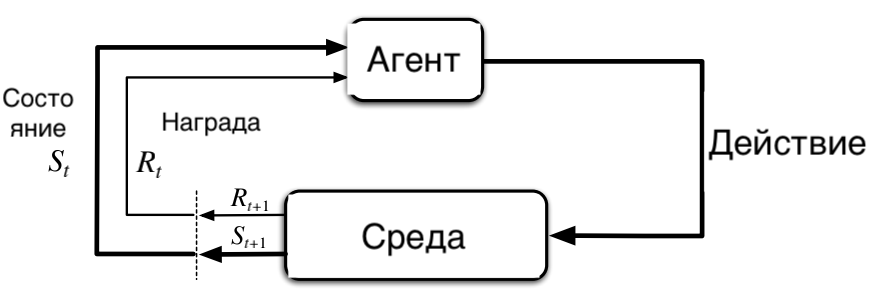
\includegraphics[width=\textwidth]{./inc/img/mdp.png}
	\caption{Марковский процесс принятия решений}
\end{figure}

Блять, если у всех наших уебков одинаково хуйовые возможности (допустим, они все игроки в онлайн шутер), то можно юзать среднюю награду за игру, как показатель того, насколько хуево они играют. А если хочется четче, то можно посмотреть на процент побед.

\pagebreak

А если нам нужно ограничить этих долбоебов, то можно настроить следующее:

\begin{itemize}[label=---]
\item количество ходов в игре --- горизонт (без жестких ограничений на время, но лучше не уебывать в ноль);
\item если наш сука агент висит, то его ебальник смотрит на нулевой вектор, а действия игнорятся;
\item действия, которые не получится сделать, маскируются и нахуй отправляются;
\item агент видит только то, что ему доступно;
\item ну и ебашим - если хотите, то обменивайтесь информацией, а если не хотите, то и не обменивайтесь.
\end{itemize}
Чтобы не допускать всяких действий, которые выражаются векторами, есть такие алгоритмы, которые называются безопасными алгоритмами обучения с подкреплением. Но это слишком сложно и мы на эту хуйню не обращаем внимание.

\subsection*{Пизданутый вывод}

Мы тут всю эту хуйню про анализ, про задачи формализования с помощью Марковских игр и прочее перетащили, но чтобы не соснуть в этой работе, нам важно еще сказать, что безопасные алгоритмы обучения с подкреплением это хуита слишком сложная для нашего гопнического ума, и мы ее не рассматривали.